\documentclass[11pt,ngerman]{article}
\usepackage{geometry}
\usepackage[T1]{fontenc}
\usepackage[utf8]{inputenc}
\usepackage{babel}
\usepackage{lmodern}%get scalable font
\usepackage{titling}
\usepackage{relsize}
\usepackage{biblatex}
\usepackage{hyperref}
\usepackage{paralist}
\usepackage[table, dvipsnames]{xcolor}
\usepackage{booktabs}
\usepackage{setspace}
\usepackage{float}
\usepackage{graphicx}
\usepackage{listings}

% Link colors
\hypersetup{
    colorlinks,
    linkcolor={blue},
    citecolor={red},
    urlcolor={blue}
}

% inline code macro
\definecolor{lightgray}{gray}{0.9}
\lstset{
    showstringspaces=false,
    basicstyle=\ttfamily,
    keywordstyle=\color{blue},
    commentstyle=\color[grey]{0.6},
    stringstyle=\color[RGB]{255,150,75}
}
\newcommand{\inlinecode}[2]{\colorbox{lightgray}{\lstinline[language=#1]$#2$}}

% Code block settings
\definecolor{codegreen}{rgb}{0,0.6,0}
\definecolor{codegray}{rgb}{0.5,0.5,0.5}
\definecolor{codepurple}{rgb}{0.58,0,0.82}
\definecolor{backcolour}{rgb}{0.95,0.95,0.92}

\lstdefinestyle{mystyle}{
    backgroundcolor=\color{backcolour},
    commentstyle=\color{codegreen},
    keywordstyle=\color{magenta},
    numberstyle=\tiny\color{codegray},
    stringstyle=\color{codepurple},
    basicstyle=\ttfamily\footnotesize,
    breakatwhitespace=false,
    breaklines=true,
    captionpos=b,
    keepspaces=true,
    numbers=left,
    numbersep=5pt,
    showspaces=false,
    showstringspaces=false,
    showtabs=false,
    tabsize=2
}
\lstset{style=mystyle}

% double quotes macro
% usage: \quotes{arg1}  => in text: "arg1"
\newcommand{\quotes}[1]{``#1''}

\geometry{a4paper, top=25mm, left=25mm, right=25mm, bottom=20mm,
    headsep=10mm, footskip=12mm}

\renewcommand{\arraystretch}{1.5}

\pretitle{\begin{center}\linespread{1.5}\huge}
    \posttitle{\par\end{center}\vspace{0.5em}}

\begin{document}

    \title{SWEN1\\Praktikum 03 GRASP\\
        \vspace{1cm}
        \small{ZHAW  School of Engineering\\Klasse: IT18tb\_zh}
        \vspace{1.5cm}
    }
    \author{
        Huber, Patrick\\
        \small{huberpa4@students.zhaw.ch}
        \vspace{1.5cm}
    }
   \date{\today}

    \maketitle
    \newpage

    \tableofcontents
    \listoffigures
    \lstlistoflistings
    \newpage

    \section{Praktikum GRASP}

    \subsection{Aufgabe 1 - Fassaden-Controller}
    Die Klasse \textbf{Forum} ist der Fassaden-Controller.

     \subsection{Aufgabe 2 - getNbrOfContributions()}
     Die GRASP Entwurfsmuster \quotes{Information Expert}, \quotes{Controller}, \quotes{Low Coupling} und \quotes{High Cohesion} wurden in dieser Aufgabe angewendet. Das Forum kennt seine Topics, diese wiederum die enthaltenen Diskussionen. Die Diskussionen wissen über ihre Contributions Bescheid. Der Fassaden-Controller \textbf{Forum} koordiniert die Anfrage des Clients. \newline
     \textit{Hinweis}: Das neue Klassendiagramm ist im \autoref{ssec:Klassendiagramm} ersichtlich.

         \subsubsection{Kommunikationsdiagramm}
          \begin{figure}[H]
             \centering
             \makebox[\textwidth][c]{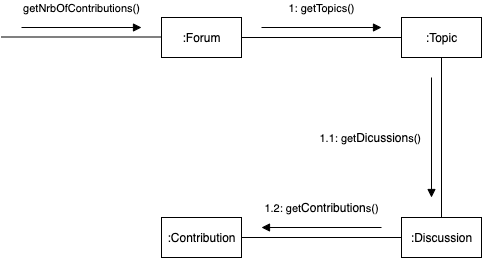
\includegraphics[width=0.85\textwidth]{figures/Kommunikationsdiagramm.png}}
             \caption{UML Kommunikationsdiagramm - getNbrOfContributions()}
             \label{fig:UMLKommunikationsdiagramm_getNbrOfContributions}
         \end{figure}

     \subsection{Aufgabe 3 - addNewDiscussion(...)}
     Die GRASP Entwurfsmuster \quotes{Information Expert}, \quotes{Controller}, \quotes{Creator}, \quotes{Low Coupling} und \quotes{High Cohesion} wurden in dieser Aufgabe angestrebt. Nur die Klasse \textbf{Topic} darf eine Discussion-Instanz erstellen. Ebenfalls weiss die Klasse \textbf{Topic} bestens über seine Discussion-Instanzen Bescheid. Der Fassaden-Controller \textbf{Forum} koordiniert die Anfrage des Clients.

        \subsubsection{Sequenzdiagramm addNewDiscussion(...)}
        \label{sssec:Sequenzdiagramm_addNewDiscussion}
        \begin{figure}[H]
            \centering
            \makebox[\textwidth][c]{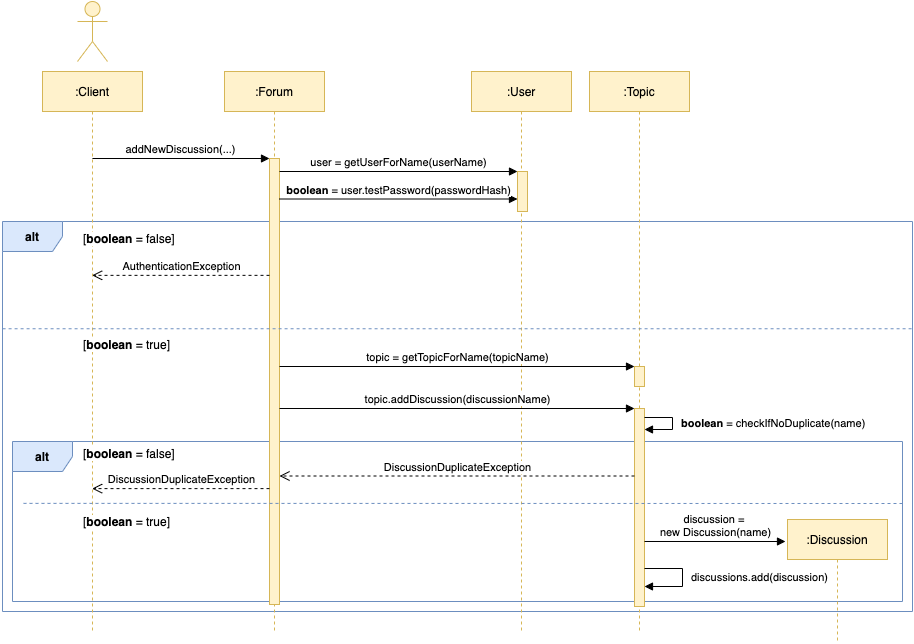
\includegraphics[width=1\textwidth]{figures/Sequenzdiagramm_addNewDiscussion.png}}
            \caption{UML Sequenzdiagramm - addNewDiscussion(...)}
            \label{fig:Sequenzdiagramm_addNewDiscussion}
        \end{figure}

     \subsection{Klassendiagramm}
     \label{ssec:Klassendiagramm}
     Das neue Klassendiagramm. Alle Neuerungen wurden mit Violett markiert.
    \begin{itemize}
        \item Neue Exception-Klasse \quotes{DiscussionDuplicateException}
        \item Die Klasse \textbf{Topic} hat zwei neue Methoden:
        \begin{itemize}
             \item \inlinecode{Java}{protected void addDiscussion(String name)}
             \item \inlinecode{Java}{private boolean checkIfNoDuplicate(String name)}
        \end{itemize}
        \item Die Klasse \textbf{Forum} hat zwei neue Methoden:
        \begin{itemize}
            \item \inlinecode{Java}{protected int getNbrOfContributions()}
            \item \inlinecode{Java}{protected void addNewDiscussion(...)}
        \end{itemize}
        \item Die Klasse \textbf{ForumTest} hat etliche neue Test-Methoden welche im \autoref{sssec:ForumTest_Code} im Detail ersichtlich sind.
    \end{itemize}
     \newpage
    \begin{figure}[H]
        \centering
        \makebox[\textwidth][c]{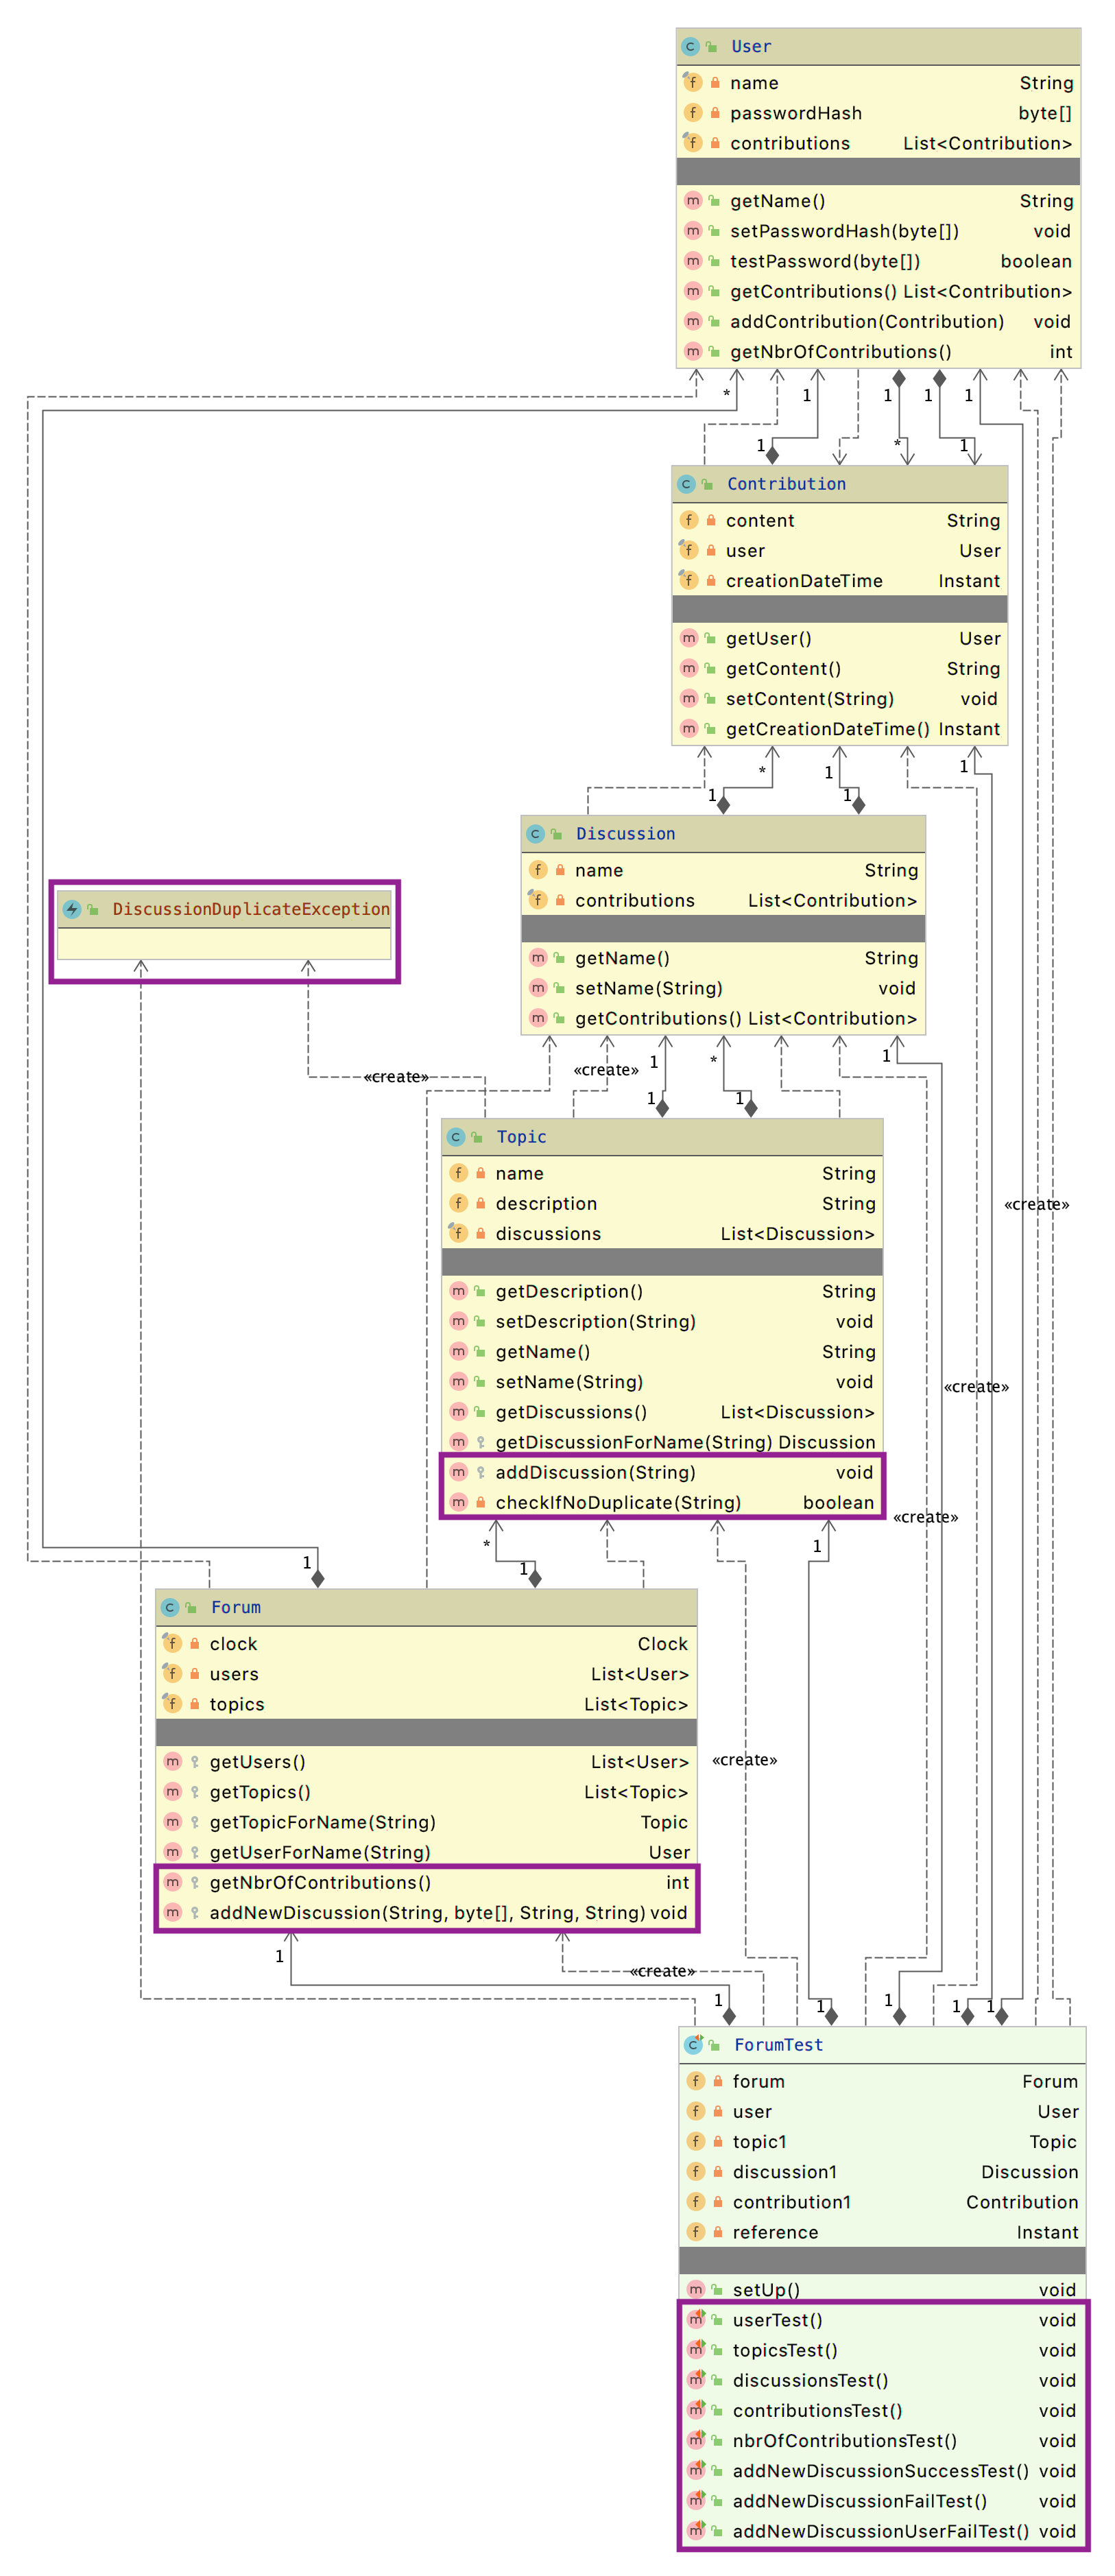
\includegraphics[width=0.65\textwidth]{figures/SWEN1_GRASP_Klassendiagramm_marks.png}}
        \caption{UML Klassendiagramm - Forum}
        \label{fig:UMLKlassendiagramm_Forum}
    \end{figure}

    \subsection{Aufgabe 4 - Neuer Code}
    \label{ssec:Codeausschnitte}
    Alle neuen Codeausschnitte sind hier aufgeführt. \newline
    \textit{Hinweis}: Der ganze Quelltext kann unter folgendem Link angesehen werden: \\ \url{https://github.zhaw.ch/huberpa4/SWEN1/tree/master/Praktikum_GRASP-FS20}

        \subsubsection{Klasse DiscussionDuplicateException}
        \lstinputlisting[language=Java, caption=Klasse DiscussionDuplicateException]{listings/DiscussionDuplicateException.code}
        \vspace{.5cm}

        \subsubsection{Klasse Topic - Methode \inlinecode{Java}{protected void addDiscussion(String name)}}
        \lstinputlisting[language=Java, caption=Klasse Topic - Methode addDiscussion(...)]{listings/Topic.addDiscussion.code}
        \vspace{.5cm}

        \subsubsection{Klasse Topic - Methode \inlinecode{Java}{private boolean checkIfNoDuplicate(String name)}}
        \lstinputlisting[language=Java, caption=Klasse Topic - Methode checkIfNoDuplicate(...)]{listings/Topic.checkIfNoDuplicate.code}
        \vspace{.5cm}

        \subsubsection{Klasse Forum - Methode \inlinecode{Java}{protected int getNbrOfContributions()}}
        \lstinputlisting[language=Java, caption=Klasse Forum - Methode getNbrOfContributions()]{listings/Forum.getNbrOfContributions.code}
        \vspace{.5cm}

        \subsubsection{Klasse Forum - Methode \inlinecode{Java}{protected void addNewDiscussion(...)}}
        \lstinputlisting[language=Java, caption=Klasse Forum - Methode addNewDiscussion(...)]{listings/Forum.addNewDiscussion.code}
        \vspace{.5cm}

        \subsubsection{Klasse ForumTest}
        \label{sssec:ForumTest_Code}
        \lstinputlisting[language=Java, caption=Klasse ForumTest]{listings/ForumTest.code}

\end{document}

